\documentclass[11pt]{article}
\usepackage{amsmath, float, graphicx, caption, subcaption}
\usepackage[a4paper,margin=1in]{geometry}

% Used to display pygraph figures
\newcommand{\smallgraph}[2]
{\begin{subfigure}[h]{2in}
	\includegraphics[width=2in]{#1}
	\caption{#2}
	\label{fig:#1}
\end{subfigure}}
\newcommand{\medgraph}[2]
{\begin{subfigure}[h]{3in}
	\includegraphics[width=3in]{#1}
	\caption{#2}
	\label{fig:#1}
\end{subfigure}}

\title{Ph 20.1 -- Introduction to Python}
\author{Ryan Burns}
\date{23 April 2015}
\begin{document}
\maketitle
\begin{enumerate}
\item
\begin{figure}[h]
\centering
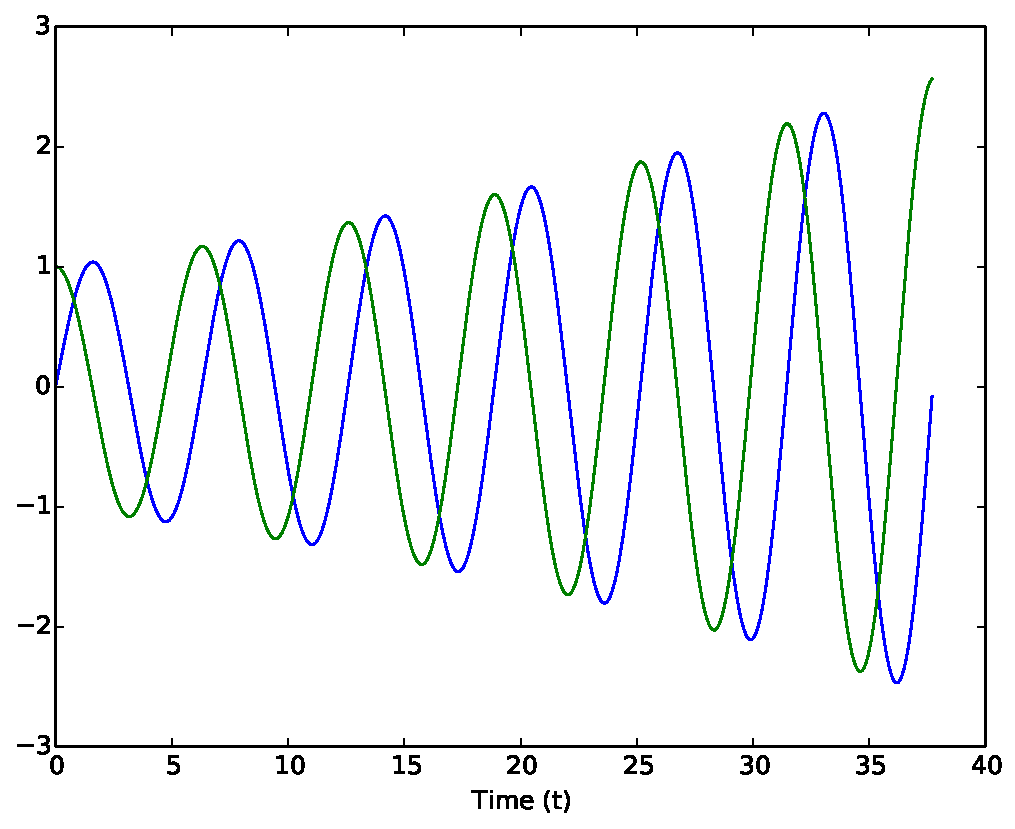
\includegraphics[width=3in]{img/explicit.pdf}
\caption{Explicit Euler method}
\end{figure}
The above graph shows the explicit Euler approximation of 6 cycles of oscillations of a mass on a spring with $k/m = 1$. The position is shown in blue, and the velocity is shown in green. A timestep of 0.05 is used, along with $x_0 = 0$ and $v_0 = 1$. As we can see, as the oscillations progress they deviate from the ideal harmonic motion we would expect due to the accumulated errors in the approximation.

\item
We can perform some algebra to construct an analytic solution to this problem. Since $k/m = 1$, the motion of the mass is described simply by $x = A \sin (t + \phi)$. We can also take the derivative of this equation to see that $v = A \cos (t + \phi)$. Given $x_0$ and $v_0$, we can solve for $\phi$ and $A$ as follows:
\begin{align*}
x_0 &= A sin \phi \\
v_0 &= A cos \phi \\
\frac{x_0}{v_0} &= \tan \phi \\
\phi &= \tan^{-1} \left( \frac{x_0}{v_0} \right) \\
A &= x_0 / \sin \phi \\
or \\
A &= v_0 / \cos \phi
\end{align*}
Plotting this analytic solution is then straightforward for any given $x_0$ and $v_0$.
\begin{figure}[h]
\centering
\medgraph{img/diff.pdf}{Euler position (blue) vs. analytical position}
\medgraph{img/error.pdf}{Error for position (blue) and velocity (green)}
\caption{Global error}
\end{figure}

\item
\begin{figure}[H]
\centering
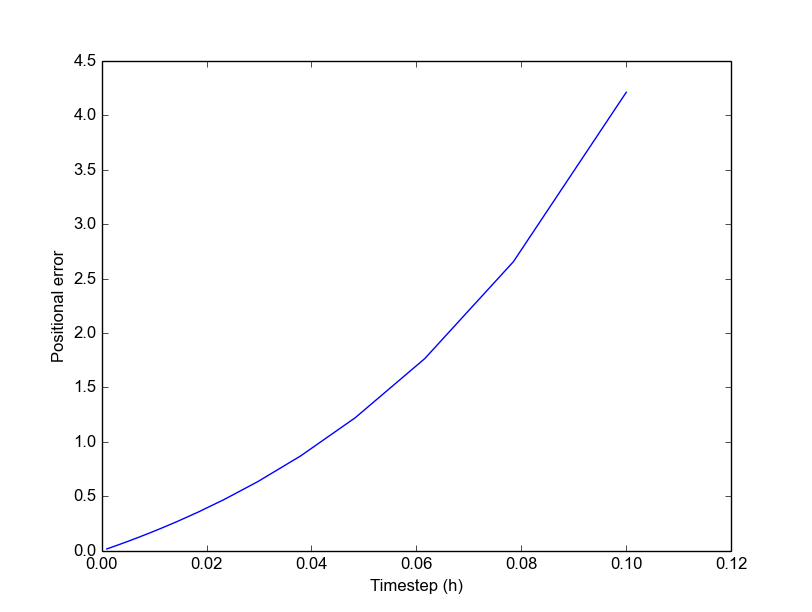
\includegraphics[width=3in]{img/truncation.pdf}
\caption{Timestep and truncation error}
\end{figure}
See above.

\item
Analytically, the energy of the system is simple. 
\begin{align*}
x^2 &= (A \sin (t + \phi))^2 = A^2 \sin^2 (t + \phi) \\
v^2 &= (A \cos (t + \phi))^2 = A^2 \cos^2 (t + \phi) \\
E &= x^2 + v^2 \\
&= A^2 \cdot \left( \sin^2 (t + \phi) + \cos^2 (t + \phi) \right) \\
&= A^2
\end{align*}
We can see that the energy of the system is constant, proportional to the amplitude of the oscillations squared. \\
The evolution of the normalized total energy follows the same trend as the evolution of the global errors, increasing at an increased rate throughout the timespan of the simulation.
\begin{figure}[H]
\centering
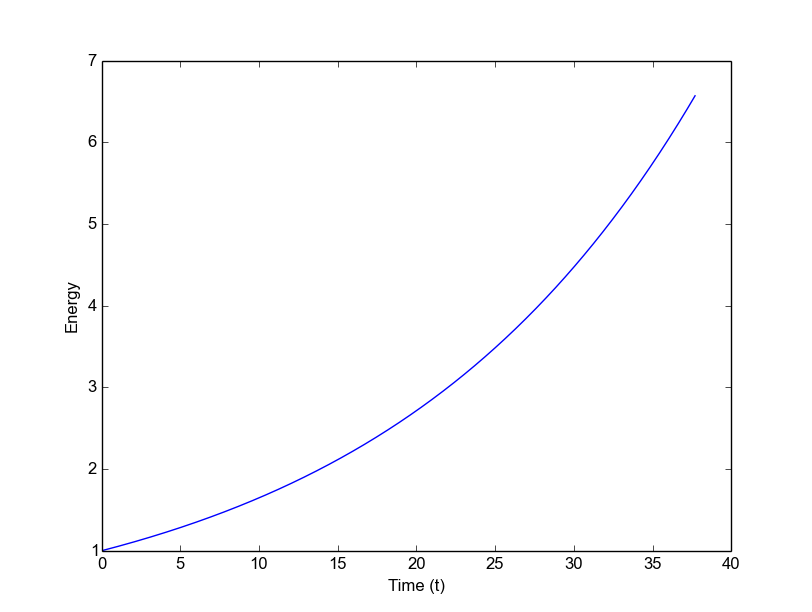
\includegraphics[width=3in]{img/energy.pdf}
\caption{Normalized total energy}
\end{figure}

\item
\begin{align*}
x_i &= x_{i+1} - h \cdot v_{i+1} \\
+ h \cdot (v_i &= h \cdot x_{i+1} + v_{i+1}) \\
= x_{i+1} \cdot (h^2 + 1) &= x_i + h \cdot v_i \\ \\
x_{i+1} &= \frac{x_i + h \cdot v_i}{h^2 + 1} \\
v_{i+1} &= v_i - \frac{h \cdot x_i + h^2 \cdot v_i}{h^2 + 1}
\end{align*}
\begin{figure}[h]
\centering
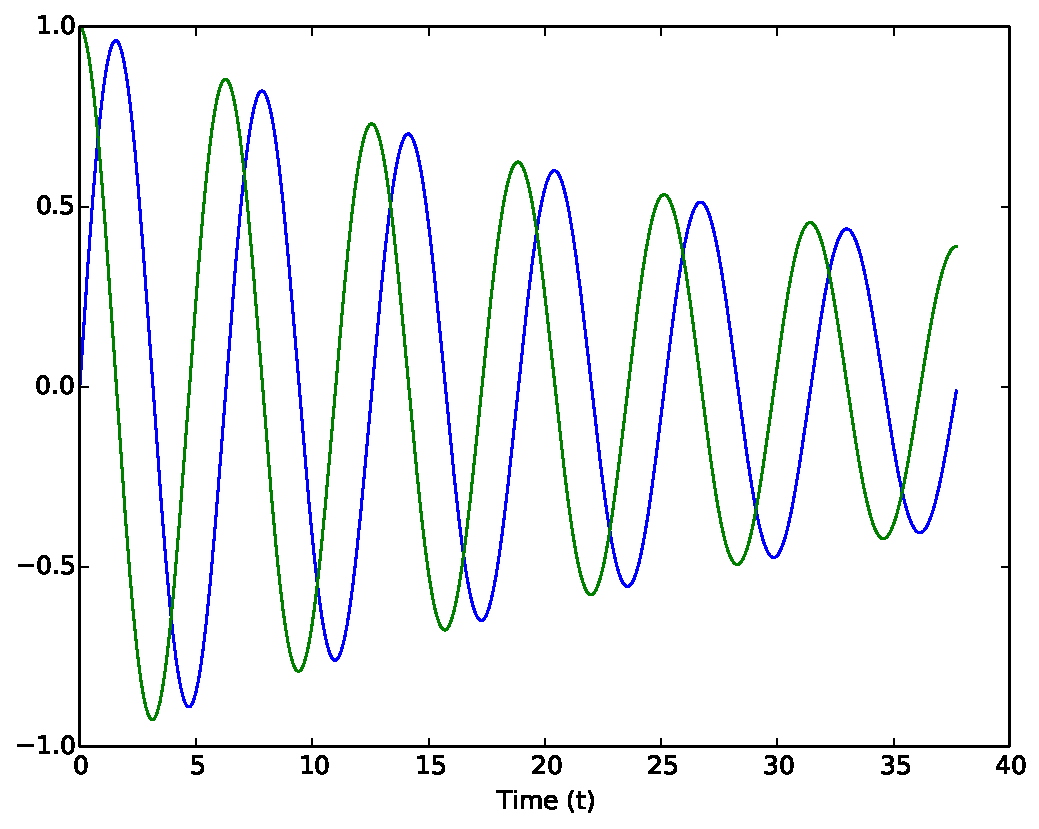
\includegraphics[width=3in]{img/implicit.pdf}
\caption{Implicit Euler method}
\end{figure}
The implicit Euler method truly is the complement of the explicit method, because the errors do the opposite of what they did before. Now the global errors cause the energy of the oscillations to decrease over time, and the function decreases its amplitude because of this. 

\end{enumerate}
\end{document}